\section{Results}

\Cref{tab:test_scores} presents the recall@10 and triplet accuracy
scores on test narration data obtained with the complete model.  In
\Cref{sec:ablations} we investigate the impact of various components
of our training setup on performance as measured by recall@10 and
triplet accuracy.  In \Cref{sec:minimal-pairs} we focus on the
targeted evaluation via minimal pairs.  

\label{sec:results}
\begin{table}[htb]
  \begin{tabular}{lll}
\toprule
R@10 (fixed) & R@10 (jitter) & Triplet Acc \\
\midrule
 0.73 ± 0.05 &   0.73 ± 0.04 & 0.91 ± 0.01 \\
\bottomrule
\end{tabular}

  \caption{Performance of the complete model on narration test
  	data. We show the mean and standard deviation over the
  	bootstrapped scores, pooled over four training runs.}
  \label{tab:test_scores}
\end{table}


\subsection{Ablations}
\label{sec:ablations}
For completeness, we report results on both dialog and narration
data. However, the scores on narration are the main focus as they are
not confounded by speaker-based clues, and thus indicate to what
extent to model learns aspects of utterance meaning.

For \Cref{fig:pretraining} we include each run as a separate boxplot
in order to illustrate the consistency of the results between runs in
different training conditions.  For the other ablations we collapse
the results of the four runs to avoid clutter.

\subsubsection{Pre-training and Fine-tuning}
Results on different pre-training configurations are shown in
\Cref{fig:pretraining}.
\begin{figure*}[htb]
	\centering
	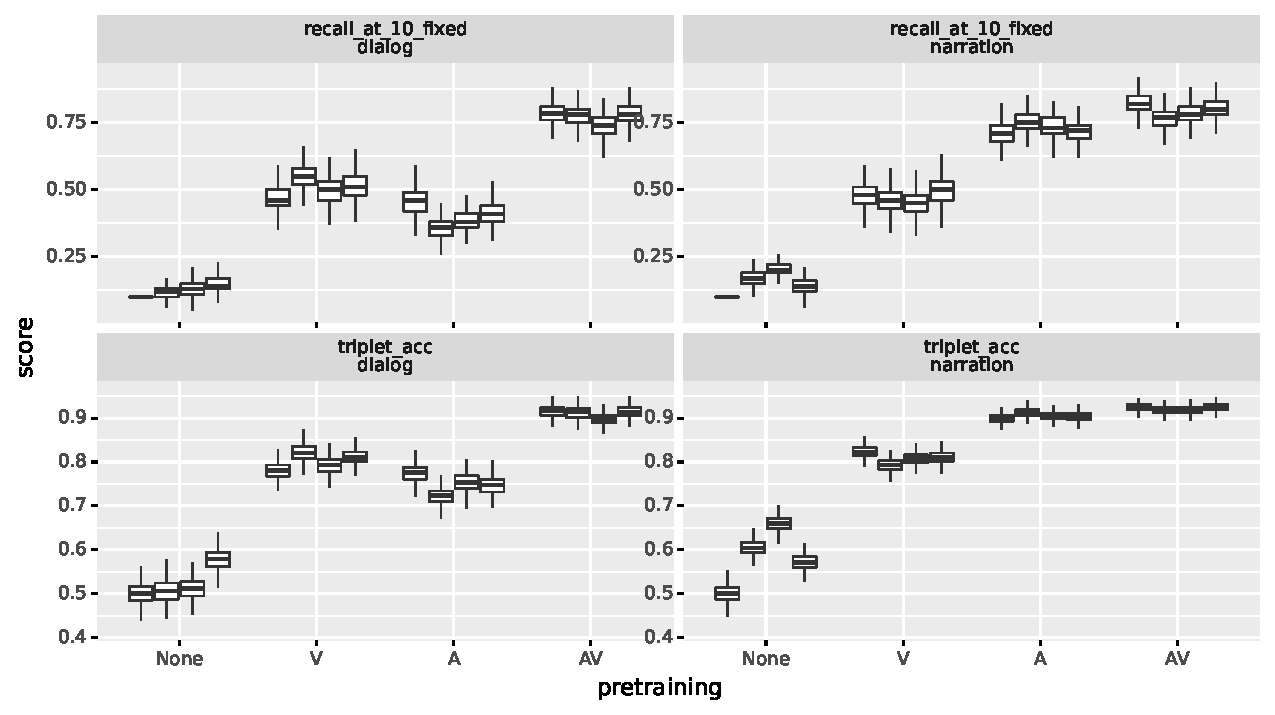
\includegraphics[width=\textwidth]{results/ablations/pretraining.pdf}
	\caption{Effect of pre-training on performance on the dialog
          and narration validation data. The top row shows recall@10
          (chance = 10\%); the bottom row triplet accuracy (chance =
          50\%). Within each condition, we show scores for four
          separate runs. AV: pretrained audio and video; A: pretrained
          audio; V: pretrained video; None: no pretraining.}
	\label{fig:pretraining}
      \end{figure*}

The best overall performance on both the dialog and the narration data is 
achieved with a model where both the video and audio encoder are pre-trained 
before being fine-tuned on our data. On narration data, for both metrics,
we see a clear ranking of
configurations from best to worst: (AV) audio and video pre-training,
(A) audio pre-training, (V) video pre-training and (None) no
trainining. Meanwhile for dialog data, the performance between A and V
is comparable. In the absence of any pre-training (None),
some runs fail to converge, thus performing at chance level.

To further understand and disentangle the effects of audio pre-training and 
fine-tuning, we train a model with frozen parameters of the 
\textsc{wav2vec} module. The effect of this condition is show in \Cref{fig:freeze_wav2vec}.
\begin{figure}[htb]
  \centering
  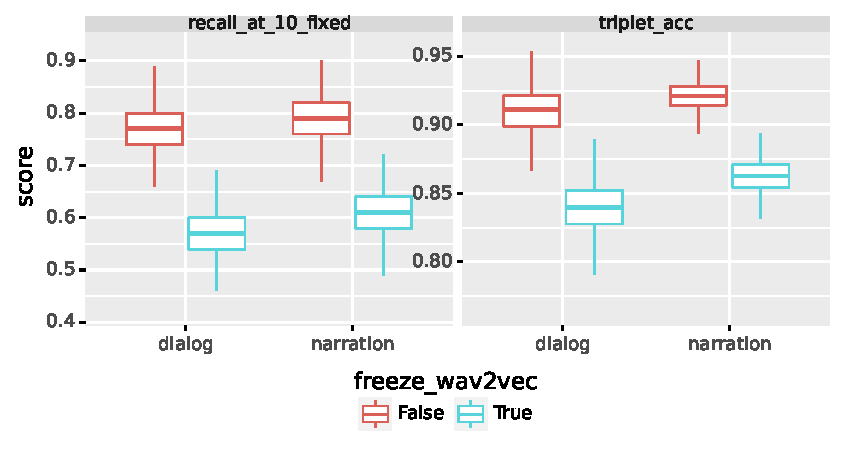
\includegraphics[width=\columnwidth]{results/ablations/freeze_wav2vec.pdf}
  \caption{Effect of freezing the parameters of the \textsc{wav2vec}
    module on model performance, on the dialog and narration
    validation data (True: \textsc{wav2vec} frozen; False:
    \textsc{wav2vec} trained). The top row
    shows recall@10; the bottom row triplet accuracy.}
  \label{fig:freeze_wav2vec}
\end{figure}
We find without fine-tuning of the \textsc{wav2vec} module, performance decreases substantially 
on both metrics. In other words, best performance is only achieved with pre-trained and 
fine-tuned models.


\subsubsection{Jitter}
Next, we evaluate a model that has been trained with varying video and audio 
lengths (\textsc{jitter}). For fair comparison, we report recall@10 for both 
\textsc{fixed} and \textsc{jitter} validation configurations.
As seen in \Cref{fig:jitter}, the effect of \textsc{jitter} is only
minor and that performance is comparable.\footnote{However, we observe 
substantial performance improvements when using \textsc{jitter} in the more 
controlled minimal pairs evaluation (cf. \Cref{sec:minimal-pairs}))}
\begin{figure}[htb]
	\centering
	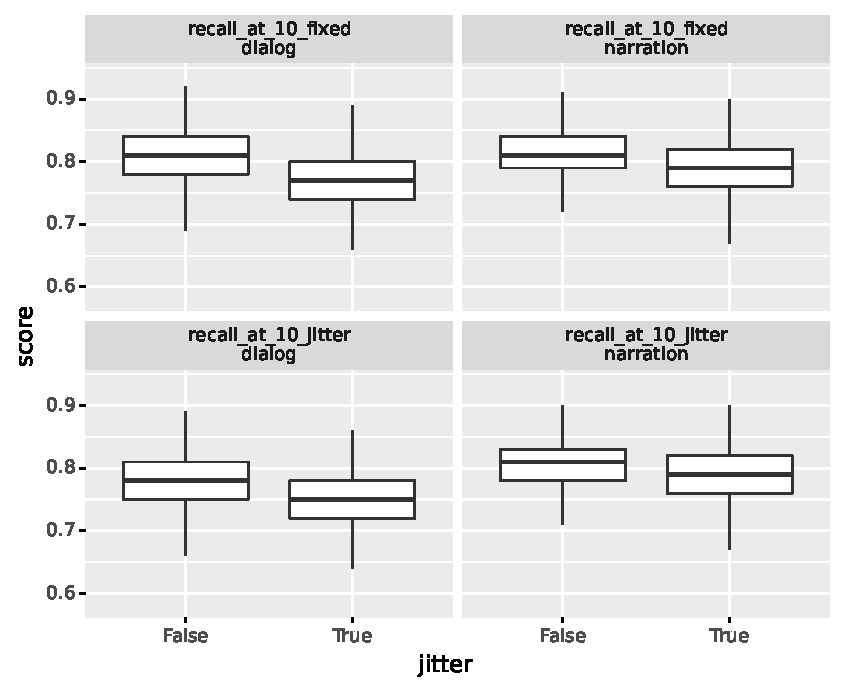
\includegraphics[width=\columnwidth]{results/ablations/jitter.pdf}
	\caption{Effect of jitter on model performance, on the dialog
          and narration validation data (True: jitter; False:
          fixed). The top row shows recall@10; the bottom row triplet
          accuracy.}
	\label{fig:jitter}
\end{figure}



\subsubsection{Temporal Information}
Finally, we explore the role of the temporal nature of the visual
modality.  \Cref{fig:static} compares the model with the regular video
encoder with one using the \textsc{static} baseline encoder.  For this
comparison we did not pre-train the video encoder in order to remove
the confound of the pre-training data.
Across
all metrics, we observe substantial performance drops for the
\textsc{static} model, which has access to the same video frames, but
does not leverage their temporal ordering. 
\begin{figure}[htb]
  \centering
  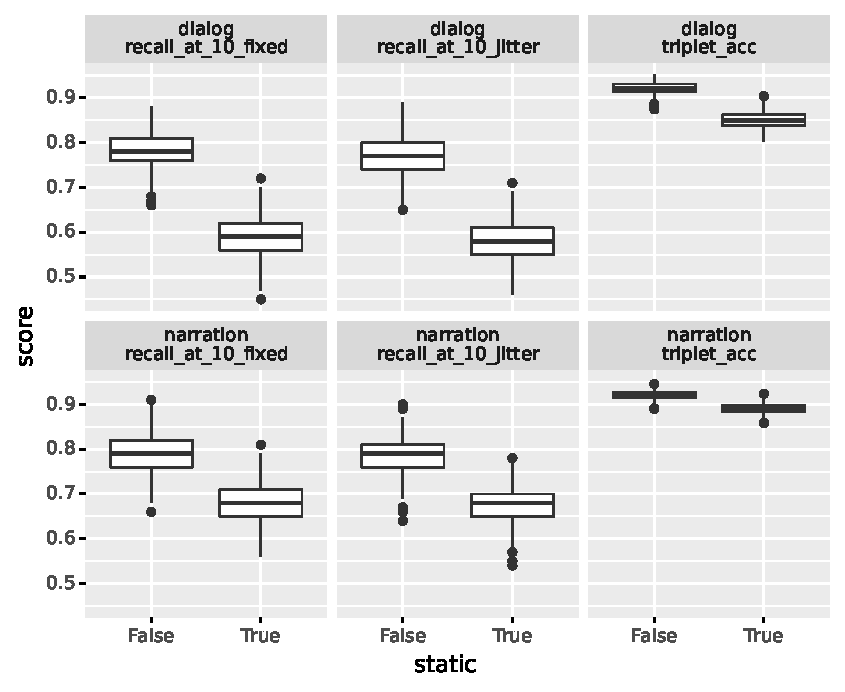
\includegraphics[width=\columnwidth]{results/ablations/static.pdf}
  \caption{Effect of a \textsc{static} image encoder on model
    performance, on the dialog and narration validation data (True:
    static video encoder; False: regular video encoder). The top row
    shows recall@10; the bottom row triplet accuracy.}
  \label{fig:static}
\end{figure}

\Cref{fig:scrambled_video} shows the effect of scrambling the video frames 
along the temporal dimension at test time. As expected, we observe substantial 
performance drops when the model does not see the video frames in 
the correct order.
\begin{figure}[htb]
	\centering
	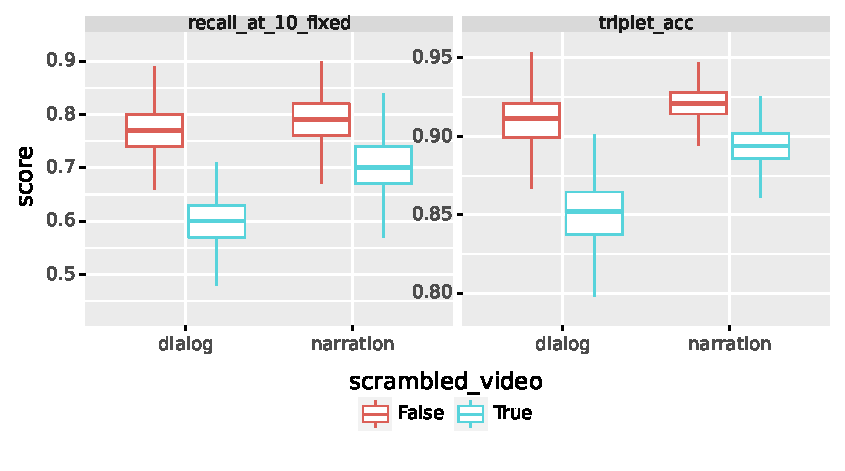
\includegraphics[width=\columnwidth]{results/ablations/scrambled_video.pdf}
	\caption{Effect of scrambling the video frames on model performance, on the 
	dialog and narration validation data (True: video frames scrambled;
        False: video frames in order). The top row shows recall@10;
		the bottom row triplet accuracy.}
	\label{fig:scrambled_video}
\end{figure}

\subsection{Minimal Pairs}
\label{sec:minimal-pairs}


\Cref{tab:minimal_pair_results} presents results for the minimal pair 
evaluation. We find that a models that are 
pre-trained and fine-tuned with \textsc{jitter} perform best. In the first two 
configurations, there is not much difference in the scores for verbs and nouns. 
However, we observe a substantial performance drop for both nouns and verbs if 
the \textsc{wav2vec} module is not fine-tuned.

If the model is trained without \textsc{jitter}, performance drops substantially
for nouns, but not for verbs. One possible explanation for this could be that 
the evaluation samples for nouns are on average shorter than those for verbs 
(nouns: $0.43s$ vs. verbs: $0.49s$), and model trained with \textsc{jitter} 
performs better on short clips because it has been exposed to clips of varying 
duration during training. Supporting this hypothesis, we find a positive 
correlation between clip duration and accuracy (Pearson $r= 0.69$, $p < 0.001$).

For a model trained on \textsc{static} data, the performance is on pair with 
the first configuration, hinting that for this task temporal information is not 
crucial. This is probably due to the fact that most evaluation samples are 
clips of rather short duration, thus not requiring much integration of 
temporal information.
\begin{table}[htb]
	\begin{tabular}{lllll}
\toprule
     Finet &       Jitt &        Tmp &      Nouns &      Verbs \\
\midrule
\checkmark & \checkmark & \checkmark & 0.81±0.002 & 0.81±0.007 \\
           & \checkmark & \checkmark & 0.71±0.002 & 0.69±0.006 \\
\checkmark &            & \checkmark & 0.73±0.003 & 0.79±0.006 \\
\checkmark & \checkmark &            & 0.79±0.002 & 0.77±0.007 \\
\bottomrule
\end{tabular}

	\caption{Minimal pair accuracies for nouns and verbs for different model 
		ablations (Finet: Finetune \textsc{wav2vec} module; 
		Jitt: \textsc{jitter}; Tmp: Temporal information (not \textsc{static})). 
		Models have been pretrained on audio and video. Mean and standard 
		deviation calculated over bootstrapped scores (100 re-samples), pooled 
		over 4 training runs.}
	\label{tab:minimal_pair_results}
\end{table}


\begin{figure}[htb]
  \centering
  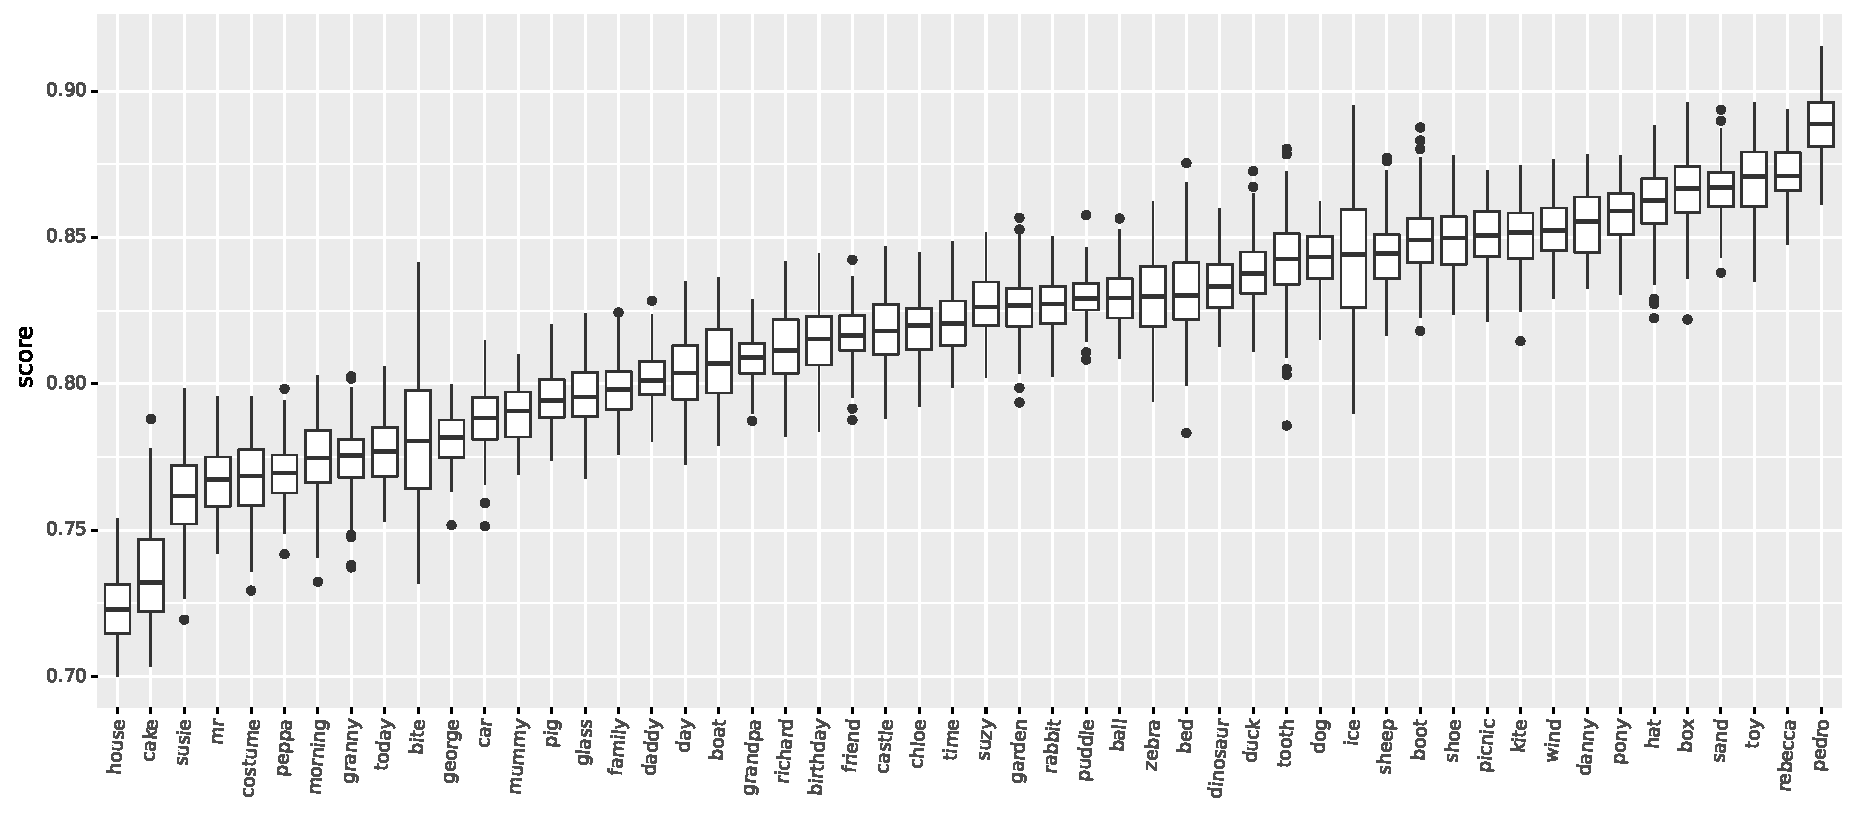
\includegraphics[width=.5\textwidth]{results/targeted_triplets/acc_per_word_NOUN.pdf}
  \caption{Per-word accuracies on the minimal pairs evaluation data for nouns.}
  \label{fig:accuracy_targeted_triplets_nouns}
\end{figure}

\Cref{fig:accuracy_targeted_triplets_nouns} shows per-word
accuracy for nouns for the best performing model configuration.
We observe substantial variance in the accuracy scores, suggesting that the 
difficulty to learn certain words varies. For example, the 
scores for ``house'', ``car'', and ``cake'' are the lowest. This could be 
because these concepts are not easy to ground, either because they are used in 
displaced speech or because they do not often refer to a similar visual entity. 
When looking at our evaluation examples, we find that indeed the word ``house'' 
is used in varying visual contexts (house entrance, whole house, inside the 
house, rabbit's house) and in displaced speech (talking about going 
to somebody's house). Cars are only sometimes completely visible, often we see 
only characters \textit{in} a car. Regarding ``cake'', it refers to either a 
whole cake, a slice, dough, or crumbs.

On the other end, performance for the concrete words such as ``ice'', ``box'', 
and ``sand'' is the best, and indeed we find that in the evaluation examples 
these concepts are always present in the corresponding video and visually 
highly similar. Additionally, the words ``Pedro'', and ``Rebecca'' 
are learned very well: They refer to ``Pedro pony'' and ``Rebecca rabbit'', 
easily visually distinguishable from other characters which are mainly pigs.

Further investigations with larger datasets are necessary to reveal the 
underlying reasons for difficulty, and relating them to predictors of age of 
acquisition in the child language acquisition literature 
\cite{roy2015predicting,frank2021variability}. 


